
C++是一个十分灵活的编程语言，其中指针的概念为程序员们提供了直接操纵内存的能力。
指针的使用使得程序员可以自由的操作内存，但是也带来了一些安全性和复杂性问题。
因此，了解程序运行的底层逻辑，对于理解C++至关重要，对于提高程序效率举重若轻，下面我们来看看C++的内存运行逻辑。

\begin{figure}[H]
    \centering
    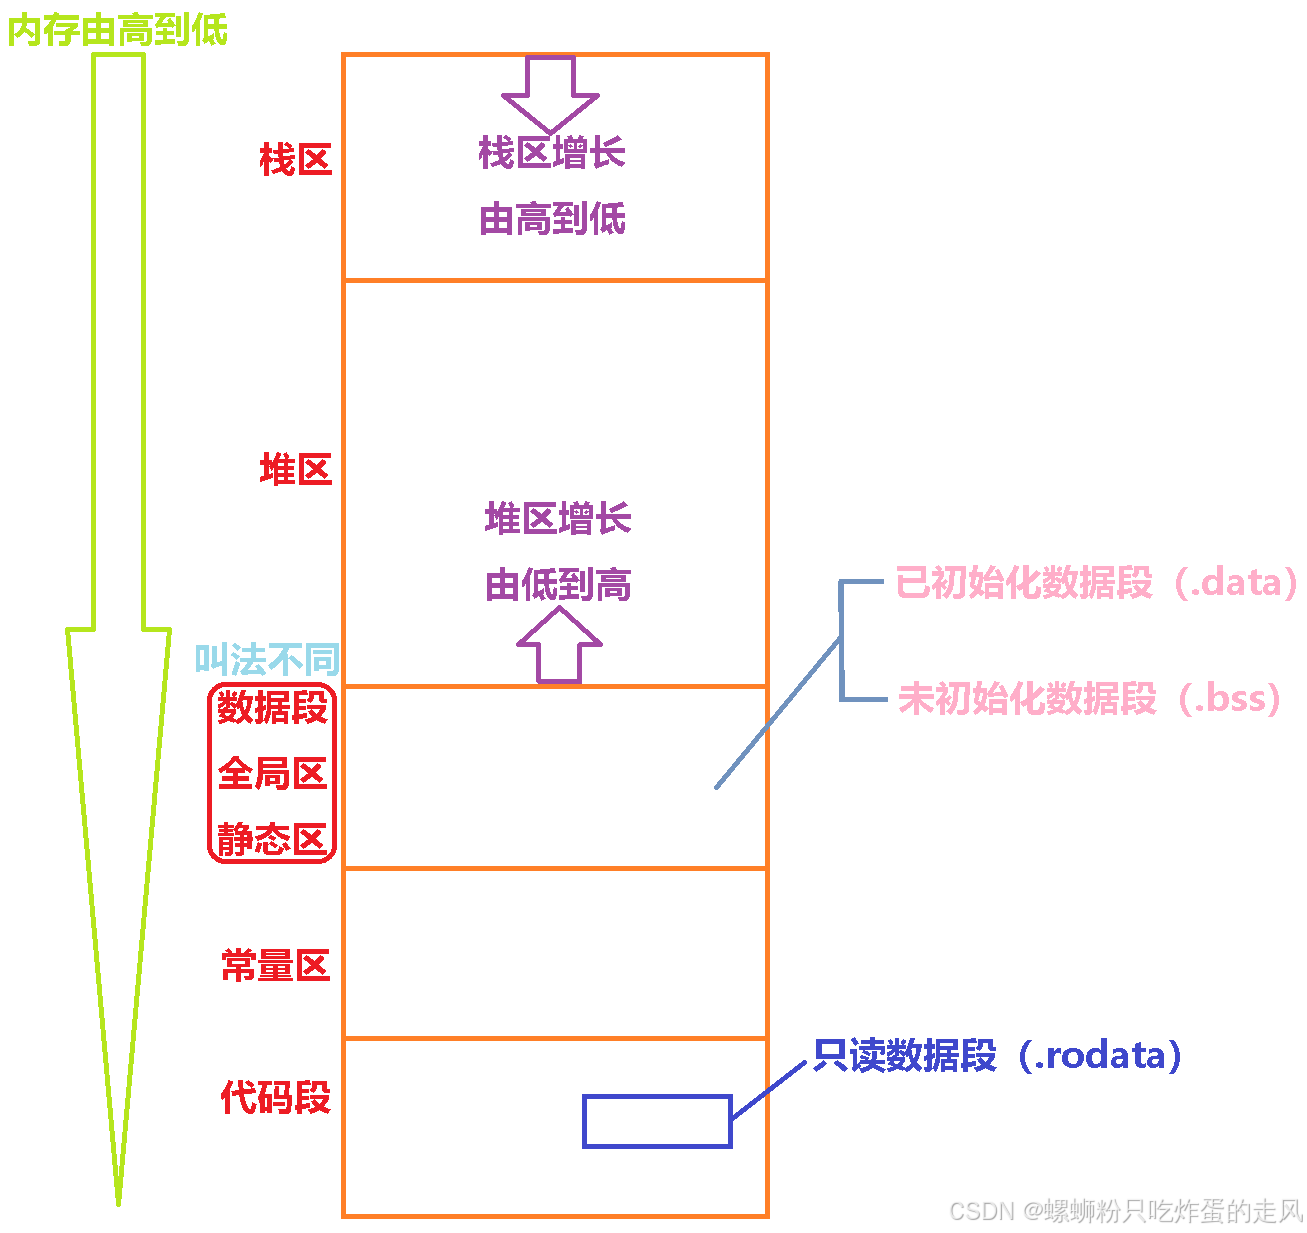
\includegraphics[width=0.7\textwidth]{系统内存.png}
    \caption{系统内存分区} % 图片标题
    \label{fig:内存分区} % 图片标签，用于引用
\end{figure}

如图\ref{fig:内存分区}，系统内存分为\textbf{代码区、常量区、全局/静态变量区、堆区、栈区等几个部分}。

\textbf{代码区和常量区}是存放程序代码和常量数据的区间一般不作区分，这里的数据是只读的，其中存储着一些在编译过程前就可以确定的数据内容
，如代码、$constexpr$修饰的变量、$const$修饰的在预编译期可以确定的值等，
一些字面常量如"Hello World!"，也存储于其中。程序在常量区中只能读取数据。

\textbf{全局/静态变量区}是存放全局/静态变量的区间，全局变量在程序运行前就已经分配了内存，静态变量在程序运行前也已经分配了内存。
但是静态变量的生命周期比全局变量长，它在程序运行结束后才释放内存。

\begin{enumerate}
    \item 全局变量：在函数外部定义的变量，它们具有全局作用域。
    \item 静态全局变量：在函数外部定义并用 $static$ 关键字修饰的变量，它们具有内部链接属性，即它们只能在定义它们的文件内部可见。
    \item 静态局部变量：在函数内部定义并用 $static$ 关键字修饰的变量，它们在函数调用结束后仍然存在，并且保持它们的值。
    \item 类静态成员变量：在类定义中使用 $static$ 关键字声明的成员变量，它们属于类而不是类的任何一个实例。
\end{enumerate}

解释一下\textbf{静态}：
\begin{enumerate}
    \item 生命周期上，静态变量在程序开始运行前或类的实例化之前就已经分配了内存，在程序运行结束后才释放内存。地址不会发生变化，就静静“躺”在静态变量区，直到程序结束。
    \item 相对于$new$的动态分配，可以让程序员选择什么时候分配和释放内存，而$static$变量则是一直存在的，直到程序结束。
    \item 静态全局变量也具有全局作用域，他与全局变量的区别在于如果程序包含多个文件的话，他作用于定义它的文件里，不能作用到其他文件里，即被$static$关键字修饰过的变量具有文件作用域。这样即使两个不同的源文件都定义了相同的静态全局变量，他们也是不同的变量。这点于全局变量不同。
\end{enumerate}

\textbf{堆区}：堆区是由程序员手动分配和释放的内存，堆区的分配和释放由\textbf{程序员控制}，程序员可以通过$new$和$delete$操作符来分配和释放内存。

在大小上，堆区的大小相对于栈区是很大的，因此可以存储更多的数据。初次之外，堆区是由程序员全权负责管理的，程序员必须小心管理堆区的分配和释放，确保程序的正确性和安全性，一般使用\textbf{智能指针}和$nullptr$判断提高程序的稳定性。
但与此同时，堆区也提供了更为灵活的编程和数据传递模式，可以参考下面的例子：
\begin{tcode}
std::vector<int>* func(){
    std::vector<int>* a = new std::vector<int>({1,2,3,4});
    std::vector<int> b{1,2,3,4};
    return a;//return &b;
    //换成return &b;之后再试试呢？
}

int main() {
    auto vecPtr = func();
    return 0;
}
\end{tcode}

\textbf{栈区}：栈区是由\textbf{编译器自动分配和释放的内存}，栈区的分配和释放都是编译器\textbf{自动完成}的，程序员\textbf{无法直接控制}栈区的分配和释放。
栈区存储数据的优势在于\textbf{快速}，但是也有一些缺点，比如栈区的大小是有限的，因此在函数调用层次过深时，可能会出现栈溢出。
栈区的大小一般是$2MB$，因此栈区的大小是有限制的，如果函数调用层次过深，可能会出现栈溢出。

\textbf{系统内存管理}：系统内存管理是操作系统的工作，它负责分配和释放系统内存，其中操作系统会自行决定栈内存，下面我们讨论一下栈区的操作。

在栈内存中，数据存储在系统栈中，只有一个开口，数据只能从栈顶入栈和出栈。在切换代码的\textbf{作用域}时，上一个作用域的数据会被新的数据压在栈的下方，
这些数据将不能被当前的程序进程所读取，直到当前的这些数据被弹出栈。
栈内存的设计是十分精妙的，它可以有效的解决内存分配和释放的问题，亦可以实现函数的层次调用，作为一名C++程序员，我们要理解透彻栈内存的运行逻辑。

\textbf{函数递归的底层原理}：函数递归是一种非常有趣的编程技巧，它可以让程序员以一种\textbf{迭代}的思想来理解和编写代码。

\begin{figure}[H]
    \centering
    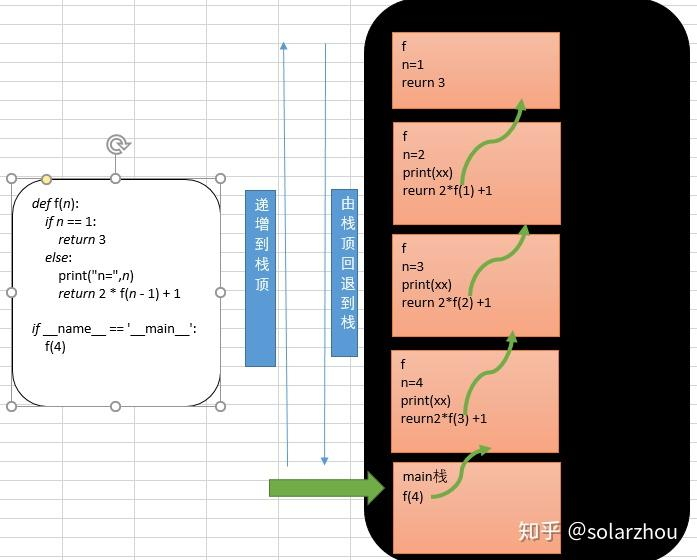
\includegraphics[width=0.7\textwidth]{栈递归.jpg}
    \caption{函数递归调用栈} % 图片标题
    \label{fig:栈递归} % 图片标签，用于引用
\end{figure}

在函数调用时，新的函数的栈帧会被压入栈中(称为栈帧)，从而覆盖掉原来的\textbf{栈帧}，当函数返回时，栈帧会被弹出栈。
露出原来的函数栈帧。当函数调用自身时，会形成一个\textbf{递归调用栈}。

需要注意的是，栈内存的大小是有限制的，当函数调用层次过深时，会出现栈溢出。

